\section{Kakas Konversi Eksperimen Pemelajaran Mesin untuk Kode Sistem}

\begin{figure}[ht]
  \centering
  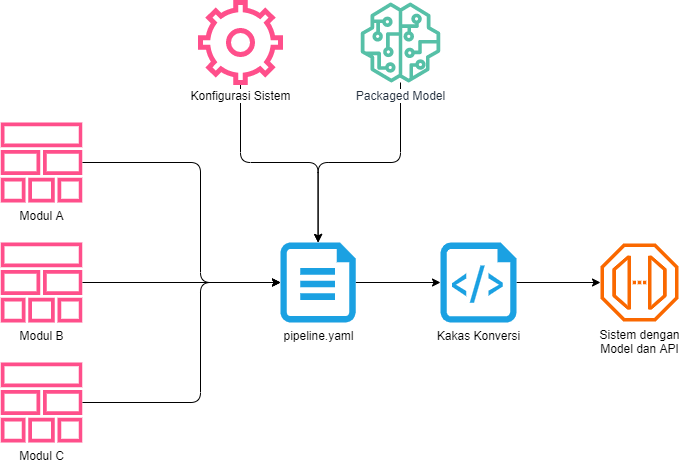
\includegraphics[width=0.7\textwidth]{03-rancangan-solusi.drawio.png}
  \caption{Rancangan Solusi Konversi Eksperimen}\label{fig:03-tool}
\end{figure}

Dalam tugas akhir ini, dibuat suatu prototipe kakas yang penulis sebut sebagai \monospace{myx} yang menggunakan hasil eksperimen yang selesai digunakan menjadi kode sistem yang siap digunakan (lihat Gambar~\ref{fig:03-tool}).
Definisi dari perjanjian data yang menjadi masukan dan keluaran akan dibuat oleh sistem secara otomatis berdasarkan eksperimen.
Alur pemrosesan yang didefinisikan dapat dibuat lewat \textit{markup file} seperti JSON atau YAML yang formatnya sudah ditentukan untuk kakas tersebut.
Alur didefinisikan lewat pemanggilan modul-modul yang diimplementasikan lebih dulu yang nantinya dapat memanggil sebuah model yang biasanya sudah siap dan disimpan dalam sebuah file.
Rincian mengenai implementasi kakas ini dapat dilihat pada Lampiran~\ref{appendix:srs}.

Selain dari konfigurasi yang didefinisikan, untuk menjalankan kakas diperlukan juga \textit{file-file} eksperimen terkait.
\textit{File-file} eksperimen yang dimaksud salah satunya adalah model hasil eksperimen.
Selain itu, \textit{file-file} eksperimen juga dapat berupa \textit{file} hasil dari eksperimen yang digunakan untuk melakukan transformasi terhadap data, misalnya seperti \textit{scaler} atau \textit{encoder} dalam eksperimen data tabular.

Modul yang dimaksud berupa potongan program yang siap untuk disatukan dengan potongan program lainnya untuk membentuk suatu sistem yang berjalan.
Modul dapat diimplementasikan dalam bahasa apapun selama semua modul yang digunakan menggunakan bahasa yang sama.
Dalam pendekatan yang umum, digunakan Docker sebagai bantuan untuk melakukan pemrosesan terhadap data.
Metode ini diterapkan dalam pengembangan eksperimen yang iteratif.
Dalam pengembangan sistem pemelajaran mesin, hal ini menjadi kurang baik karena akan memerlukan komputasi yang lebih berat akibat penggunaan \textit{containerization} yang pada dasarnya tidak diperlukan.

Hasil akhir dari kakas ini adalah sebuah kode sistem yang siap digunakan untuk \textit{production} yang terbentuk dari konfigurasi masukan seperti modul-modul yang dinginkan.
Kakas ini bersifat \textit{non-domain specific} atau dapat digunakan untuk kasus pembuatan sistem inferensi secara umum.
Pemilihan \textit{interface} untuk model ditentukan lewat \textit{markup file} yang telah dibuat.
Metode komunikasi yang akan diimplementasikan adalah REST sebagai contoh dari \textit{interface} yang umum digunakan dalam sistem.

Penulis mengimplementasikan kakas ini dalam bahasa Go.
Pemilihan bahasa didasarkan kepada \textit{library} yang tersedia dalam bahasa tersebut dan bahasa Go yang bersifat \textit{strong-typing} untuk memastikan struktur program yang baik.
Hasil dari proses konversi yang dilakukan kakas akan berupa kode program dalam bahasa Python dengan \monospace{FastAPI}.

